\documentclass{article}
\usepackage[utf8]{inputenc}
\usepackage[margin=1in]{geometry}
\usepackage{cite}
\usepackage{amsmath,amscd, amssymb}
\usepackage{dsfont}
\usepackage{bbm}
\usepackage{mathtools}
\usepackage{graphicx}
\graphicspath{{figures/}}
\usepackage{caption}
\usepackage{subcaption}
\usepackage{float}
\usepackage{hyperref}
\usepackage{dirtytalk}
\usepackage{multicol}
\usepackage{url}

\title{\LARGE \textbf{Hapmix: Local Ancestry Inference with HMM}}
\author{Yilei Huang yh362}
\date{December 2019}

\begin{document}

\maketitle

\section{Introduction}
    Admixture is a common theme in population genetics. The genomes of admixed individuals are composed of segments of distinct ancestral origins. It is of intrinsic interest for population genetics to infer local ancestry in these mosaic genomes; in addition, it is of great utility some real world applications, such as disease gene mapping.  

    This final project is a re-implementation of the Hapmix model proposed in 2009\cite{hapmix}. With phased SNP data of ancestral populations, Hapmix uses a hidden markov model to infer local ancestry of admixed individuals. For the haploid model presented here, it assumes that we have phased genotype data for both the reference population and the admixed individuals. It also assumes that there is only a single admixture event and the admixed individuals possess only two ancestral populations. 
\section{The Hapmix Model}
    The transition model used in Hapmix was deeply rooted in the model for linkage disequilibrium first propsoed by Li and Stephen in 2003 \cite{Li and Stephen}. In Li and Stephen's model, given a set of haplotype $\{h_1,\cdots,h_k\}$, the next observed haplotype, $h_{k+1}$, is an imperfect mosaic of the first $k$ observed haplotypes (Fig.\ref{fig:Li}). The model assumes that the copying process is first-order Markov along the chromosome, and the recombination event is a Poisson process (thus the distance between each event follows an exponential distribution with the same rate). 
    
    \begin{figure}[H]
        \includegraphics[width=8cm]{Li&Stephen.jpg}
        \centering
        \caption{A Graphical Representation of Hapmix \cite{Li and Stephen}} \label{fig:Li}
    \end{figure}
    
    
    Building upon Li and Stephen's model, in Hapmix, we assume that we have two sets of phased ancestral haplotypes, $P1$ and $P2$ and phased haplotypes of the admixed individuals. For simplicity, assume all haplotypes have valid data at the same set of SNP sites. An admixed haplotype can be seen as an (imperfect) copying process from $P1$ and $P2$, with certain transition and emission probabilities to be discussed below (Fig.\ref{fig:hapmix}). 
    
    \begin{figure}[H]
        \includegraphics[width=8cm]{hapmix.png}
        \centering
        \caption{A Graphical Representation of Hapmix \cite{hapmix}} \label{fig:hapmix}
    \end{figure}
    
    
    Assume the admixture event occurred at a single time $T$ generations ago, with $\mu_1,0<\mu_1<1$ of the admixed haplotype drawn from $P1$ and $1-\mu_1$ drawn from $P_2$. We model ancestry switches along the chromosome as Poisson process at a rate $T$ per genetic distance; therefore, the distance between each ancestry switches should follow an exponential distribution with rate $T$ per genetic distance. Let $r_s$ denote the genetic distance between site $s_{r-1}$ and $s_r$, then recombination in this segment has rate $r_sT$, thus the probability of there having an ancestry switch (which implies a recombination event) is $1-e^{-r_sT}$. Using different rate parameters, We model recombination within the same ancestral population in exactly the same way. We model switches between individuals within $P1,P2$ as a Poisson process with rate $\rho_1,\rho_2$, respectively. Similarly, the probability of there having a switch between individual haplotype in a segment of length $r_s$ is $1-e^{r_s\rho_l},l\in \{1,2\}$.  
    
    
    
    
\subsection{A Simple Haploid Model without Miscopying}

Suppose we have $k_1,k_2$ phased haplotypes sampled from reference ancestral population $P1,P2$. The hidden state in the HMM can be specified as a Cartesian product between ancestral population and individuals within that ancestral populations. More concretely, a hidden state $(i,k)$ means that, this SNP site is copied (potentially imperfect due to mutation, genotyping errors, etc) from haplotype $k$ in population $i(i\in \{1,2\})$. Then, the transition probability can be naturally specified as follows (this is a simplication of the transition probability introduced in the original Hapmix paper \cite{hapmix} by disallowing miscopying and setting $p_l=0$):

\[
P(s_j=(l,n)|s_{j-1}=(i,k))=
\begin{dcases}
\left(1-e^{-r_jT}\right)\mu_l\frac{1}{n_l}, &i\neq l\\
\left(1-e^{-r_j T}\right)\mu_l\frac{1}{n_l}+e^{-r_j T}\left(1-e^{-\rho_l r_j}\right)\frac{1}{n_l}, &i=l \land k\neq n\\
e^{-r_j T}e^{-\rho_l r_j}+\left(1-e^{-r_j T}\right)\mu_l\frac{1}{n_l}+e^{-r_j T}\left(1-e^{-\rho_l r_j}\right)\frac{1}{n_l}, &i=l \land k= n
\end{dcases}
\]

For emission probability, we specify the mutation parameter for $P1,P2$ by $\theta_1,\theta_2$, respectively. As explained in the original paper, there is good reason to scale these two parameters by the number of haplotypes in each reference population, so they will be different in most cases. Denote the genotype of site $j$ in individual $k$ in population $i$ as $h_{ik}(j)$. Let the genotype of the admixed haplotype at site $j$ as $s_j$, then
\[
e_{(i,k)}(s_j)=(1-\theta_i)\mathbbm{1}_{s_j=h_{ik}(j)}+\theta_i \mathbbm{1}_{s_j \neq h_{ij}(j)}
\]


\subsection{A More Realistic Haploid Model with Miscopying}

The original Hapmix paper \cite{hapmix} describes a somewhat more sophisticated model that allows a particular site originating from one population to copy from the other ancestral population with probability $p$. They observed that this additional complication greatly improves the performance of the model, and they have based their argument on incomplete lineage sorting and deep coalescence time. I have implemented both models with and without miscopying and will compare their performances in the third section.

In this miscopying model, the hidden state $(i,j,k)$ is specified by a triplet: $i$ represents the ancestry at this site, $j$ is the ancestry where this allele copies from (note $j$ may be different from $i$ in this miscopying model), and $k$ is the individual haplotype in population $j$ from which the allele gets its copy. The transition probability is given by the following set of equations \cite{hapmix}:

\[P(s_d=(i,j,k)|s_{d-1}=(l,m,n))=\]
$$\begin{dcases}
\left(1-e^{-r_d T}\right)\mu_l\frac{1-p}{n_m}, & l\neq i \land m=l\\
\left(1-e^{-r_d T}\right)\mu_l\frac{p}{n_m}, & l\neq i \land m\neq l\\
e^{-r_d T}\left(1-e^{-r_d \rho_l}\right)\frac{1-p}{n_m}+\left(1-e^{-r_d T}\right)\mu_l \frac{1-p}{n_m}, & l=i \land m=l \land (j\neq m \lor k\neq n)\\
e^{-r_d T}e^{-r_d \rho_l}+e^{-r_d T}\left(1-e^{-r_d \rho_l}\right)\frac{1-p}{n_m}+\left(1-e^{-r_d T}\right)\mu_l \frac{1-p}{n_m}, & l=i \land m=l \land j= m \land k=n)\\
e^{-r_d T}(1-e^{-r_d \rho_l})\frac{p}{n_m}+(1-e^{-r_d T})\mu_l\frac{p}{n_m}, & l=i \land m\neq l \land (j \neq m \lor k \neq n)\\
e^{-r_d T}e^{-r_d \rho_l}+e^{-r_d T}(1-e^{-r_d \rho_l})\frac{p}{n_m}+(1-e^{-r_d T})\mu_l\frac{p}{n_m}, & l=i \land m\neq l \land j=m \land k=n\\
\end{dcases}$$

A few words about the miscopying probability $p$. In the original paper\cite{hapmix}, there is a $p_l$ parameter for the two ancestral populations separately. To keep it simple, I have used a single $p$ in my implementation. In fact, in all the simulations and applications of Hapmix described in the original paper\cite{hapmix}, $p_l$ is the same $\forall l$, effectively using only a single value of miscopying probability.

For the emission probability, let $s_d$ be the genotype of the admixed haplotype at site $d$. As before, denote the mutation parameter for $P_1,P_2$ by $\theta_1,\theta_2$, and let $\theta_3$ be the mutation parameter for miscopying (for simplicity, $\theta_3$ is independent of the true ancestry. We just use a single value for both ways).

\[
e_{(i,j,k)}(s_d)=
\begin{dcases}
(1-\theta_j)\mathbbm{1}_{s_d=h_{jk}(d)}+\theta_j\mathbbm{1}_{s_d\neq h_{jk}(d)},&i=j\\
(1-\theta_3)\mathbbm{1}_{s_d=h_{jk}(d)}+\theta_3\mathbbm{1}_{s_d\neq h_{jk}(d)},&i\neq j
\end{dcases}
\]


\subsection{Runtime Complexity}

The standard approach for a forward-backward calculation takes time $O(k^2n)$, where $k$ is the number of hidden states and $n$ the length of the haplotype. Assume we have phased haplotype of $n_1,n_2$ individuals from $P1,P2$, respectively. In the simpler model without miscopying, $k=n_1+n_2$, and in the model with miscopying, $k=2(n_1+n_2)$. Although this is not a terribly slow implementation, a naive DP calculation of forward-backward matrix is still computationally intensive. I first implemented the simpler model in the standard approach, for $k\approx 400$ and $n=114600$, a single round of forward-backward computation plus posterior probability calculation takes $\sim 2000s$ with $\sim 30$ cores (I coded each iteration of forward-backward into matrix form, with numpy, different blocks of a matrix are computed in parallel automatically). I profiled the code, which revealed that scipy.special.logsumexp takes more than $60\%$ computing time. With suggestions from Amy, later I modified the iteration in forward-backward based on the fact that many terms in the transition probability are shared across many entries, and I only need to compute one of them, which eliminates many of the redundant logsumexp steps. In theory, this new approach should take time $O(kn)$, which is indeed consistent what I have observed. For the model without miscopying, it takes $\sim 200s$ on a single core to finish a forward-backward step, and $\sim 420s$ for the model with miscopying. This indicates that the running time is indeed linear with respect to $k$.

\section{Results}
    Phased haplotypes of chromosome 1 of Utah residents with Northern and Western European ancestry from the CEPH collection (CEU) and Yoruba in Ibadan, Nigeria (YRI) were downloaded from Hapmap3 project website \cite{hapmap3}. Trios, duos and unrelated haplotypes were combined and a subset of them (101 haplotypes) were randomly selected and used in simulating admixed haplotypes with admix-simu program from Williams Lab github. The remianing haplotypes were used as reference panel in Hapmix inference. A total of 114,600 SNP sites were retained after filtering to include only biallelic sites for inference.
    
    To explore how Hapmix performs under different admixture time, 100 admixed haplotypes were simulated for each of $T=6,20,50,100$ generations with CEU ancestry comprising of 20\% of the ancestry. For each SNP site, posterior probability of having ancestry from CEU was calculated and used for analysis presented below.
    
\subsection{Comparison between Haploid Model with and without Miscopying}
    For this subsection, miscopying probability was set to 0.05, as described in the original paper \cite{hapmix}. Since CEU was the minor ancestry in the simulation, only sites with posterior probability greater than 90\% were inferred to have ancestry from CEU. For each admixed haplotype, the hamming distance between inferred ancestry and true ancestry was calculated.
    
    \begin{figure}[H]
     \centering
     \begin{subfigure}[b]{0.45\textwidth}
         \centering
         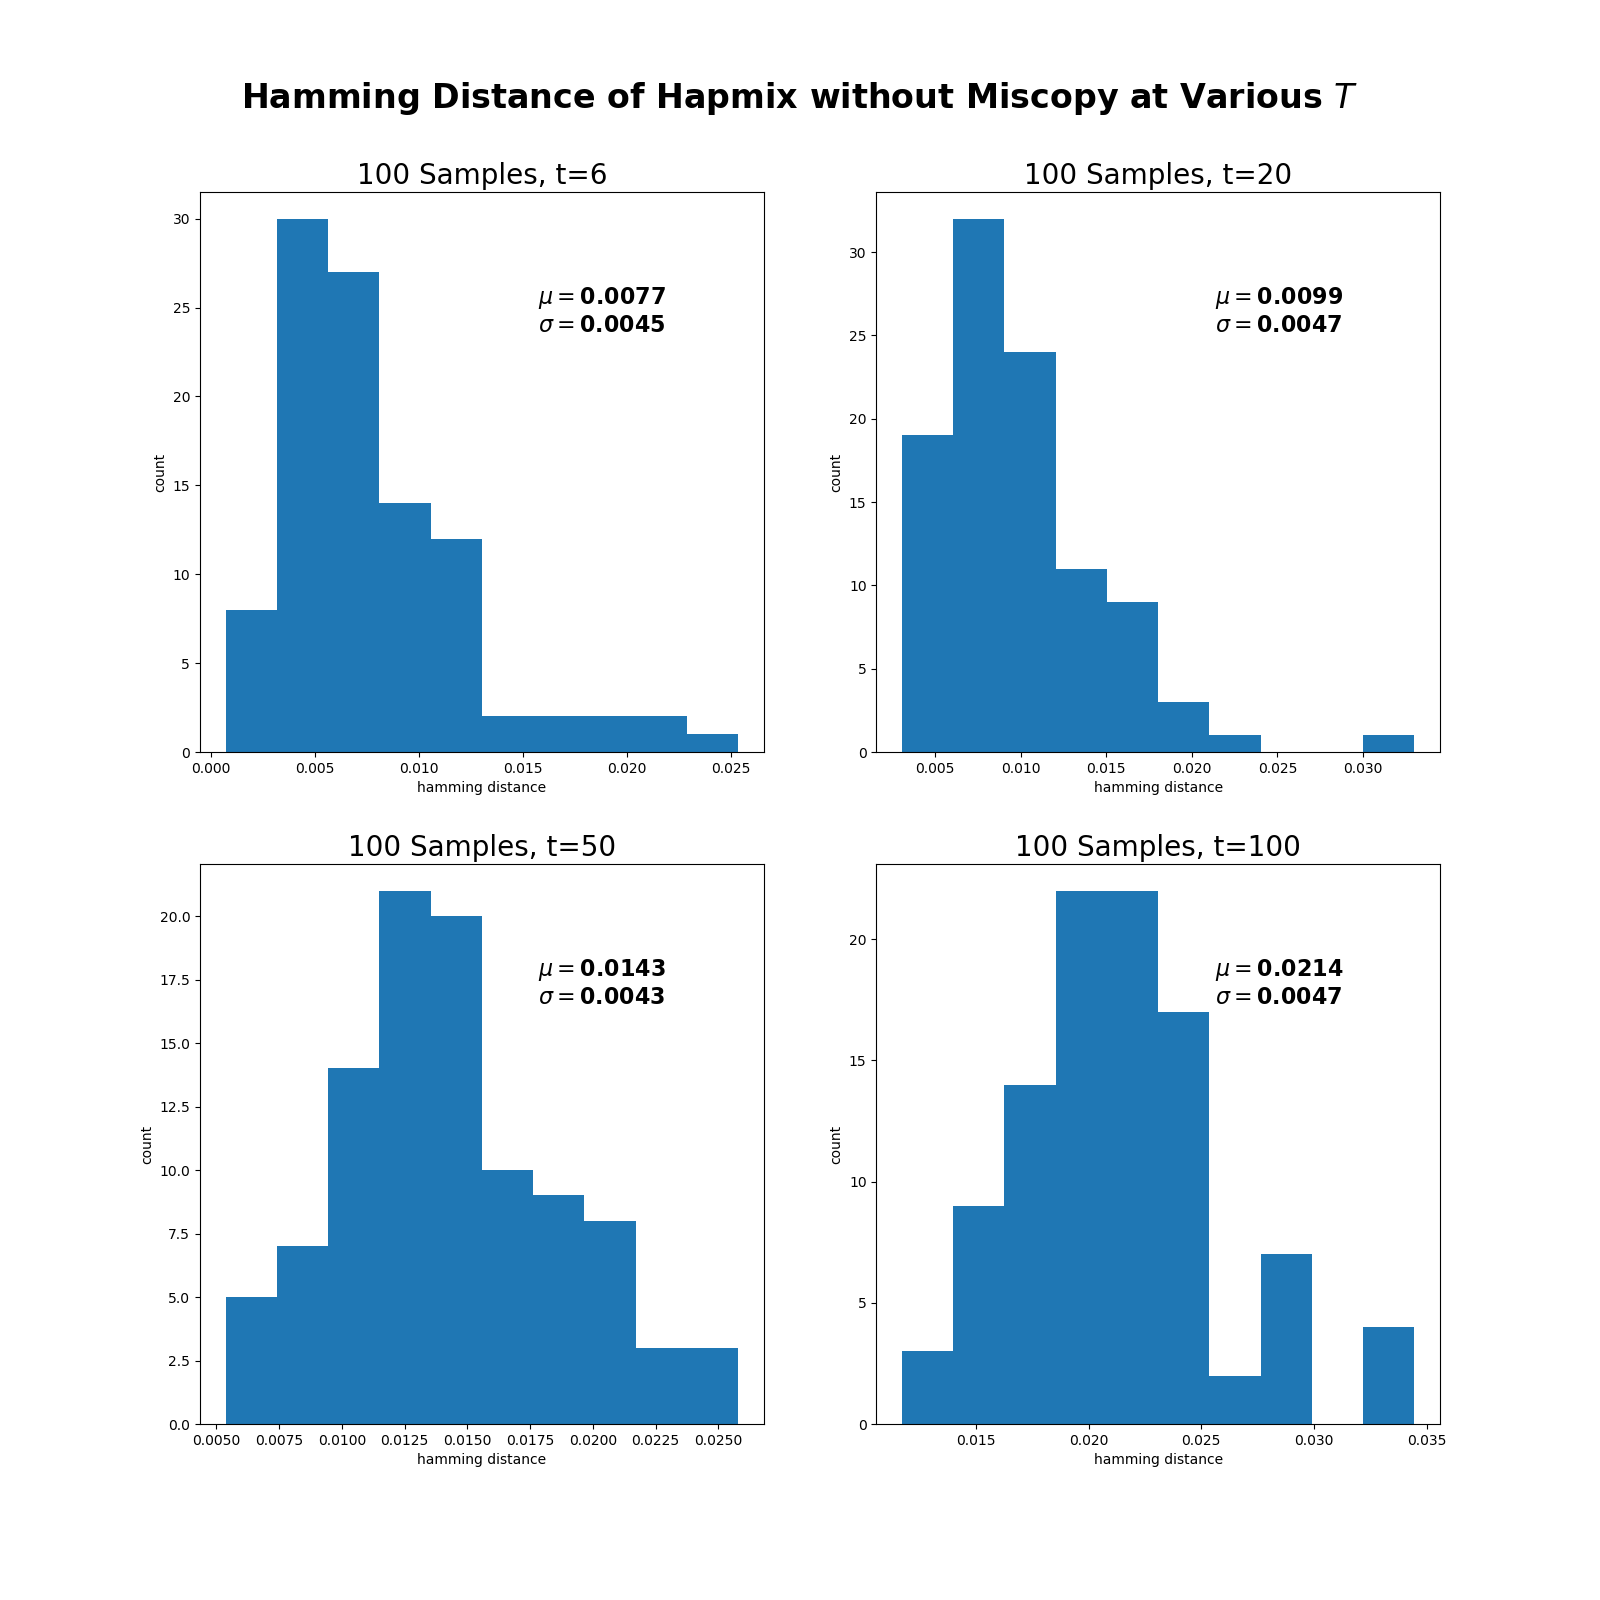
\includegraphics[width=\textwidth]{hamDist_noMiscopy.png}
         \caption{Hapmix without miscopying}
         \label{fig:nomiscopy}
     \end{subfigure}
     \hfill
     \begin{subfigure}[b]{0.45\textwidth}
         \centering
         \includegraphics[width=\textwidth]{hamDist_miscopy=5.png}
         \caption{Hapmix with miscopying $=0.05$}
         \label{fig:miscopy}
     \end{subfigure}
        \caption{Histogram of Hamming Distance between Predicted and True Ancestry}
        \label{fig:ham distance}
\end{figure}
    
     \begin{figure}[H]
     \centering
     \begin{subfigure}[b]{0.45\textwidth}
         \centering
         \includegraphics[width=\textwidth]{noMiscopy6.png}
         \caption{Hapmix without miscopying, $T=6$}
         \label{fig:noMiscopy6}
     \end{subfigure}
     \hfill
     \begin{subfigure}[b]{0.45\textwidth}
         \centering
         \includegraphics[width=\textwidth]{miscopy6.png}
         \caption{Hapmix with miscopying $=0.05$, $T=6$}
         \label{fig:miscopy6}
     \end{subfigure}
     \vfill
     \begin{subfigure}[b]{0.45\textwidth}
         \centering
         \includegraphics[width=\textwidth]{noMiscopy100.png}
         \caption{Hapmix without miscopying, $T=100$}
         \label{fig:noMiscopy100}
     \end{subfigure}
     \hfill
     \begin{subfigure}[b]{0.45\textwidth}
         \centering
         \includegraphics[width=\textwidth]{miscopy100.png}
         \caption{Hapmix with miscopying $=0.05$, $T=100$}
         \label{fig:miscopy100}
     \end{subfigure}
        \caption{Histogram of Hamming Distance between Predicted and True Ancestry}
        \label{fig:posterior}
\end{figure}
    
    
    
    
    Fig.\ref{fig:ham distance} shows the distribution of hamming distance of 100 simulated haplotypes for the four different $T$ values. Several simple observations can be made regarding Hapmix's performance. First, for both Hapmix with and without miscopying, bias increases with $T$. For relatively small $T$ values ($T=6,20$ in this case), Hapmix with miscopying yields smaller bias compared to Hapmix without miscopying. For larger $T$ values, however, Hapmix without miscopying has smaller bias. This is potentially due to the fact that, when $T$ value is small, each block of ancestry is relatively large. Hapmix without miscopying tends to produce lots of spurious ancestry switches that are very short. Hapmix with miscopying can correct these false positives. When $T$ value is large, however, many of the true positives are in fact very small, and Hapmix with miscopying produces false negatives for these very small regions of ancestry switches. Fig.\ref{fig:posterior} shows the posterior probability across all 114,600 SNP sites along the chromosome 1. Shaded region indicates true ancestry origin of CEU. Comparing Fig.\ref{fig:noMiscopy6} and Fig.\ref{fig:miscopy6}, it can be seen that all of the false positives in Fig.\ref{fig:noMiscopy6} was eliminated by the miscopying process in Fig.\ref{fig:miscopy6}. Comparing Fig.\ref{fig:noMiscopy100} and Fig.\ref{fig:miscopy100}, the Hapmix with miscopying process flags some of the true ancestry switches (indicated by red arrows) as false negatives, which potentially explains why miscopying Hapmix has higher bias when $T$ is large.
    
    To calibrate the posterior probability, the posterior probabilities were binned at bin size 0.05, and for each bin, we count the frequency with which SNP sites that fall into that bin have true ancestry origin from CEU Fig.\ref{fig:calibrate}. Unfortunately, neither my implementation of haploid Hapmix with miscopying nor Hapmix without miscopying seem to have good probability calibration. Furthermore, the posterior probability produced by Hapmix is almost consistently overestimating the true frequency, except for the two most extreme bins. That said, the majority of SNP sites fall into the first and last bins. For $T=6,20,50,100$, running Hapmix with miscopying=0.05, 99.19\%, 98.03\%, 95.51\%, 91.9\% of SNP sites in the simulated 100 haplotypes fall in either $(0,0.05)$ or $(0.95, 1)$, respectively. For Hapmix without miscopying, the percentages are 99.06\%, 98.47\%, 97.42\%, 95.81\% respectively. The fact that posterior probabilities are particularly off the reference for intermediate-valued bins shows that Hapmix has some difficulties in estimating boundaries of ancestry switches, which is somewhat expected given the nature of Hidden Markov Model. The decreasing percentage of SNPs falling into the two most extreme bins as T increases is yet another manifestation of Hapmix's difficulty in resolving highly mosaic local ancestry, consistent with our previous observation that bias increases as $T$ increases. It came as a surprise that $T=100$ produces the best probability calibration in the four values tested, especially for Hapmix with miscopying, given that local ancestry inferred by Hapmix is more biased when $T$ is large.
    
     \begin{figure}[H]
     \centering
     \begin{subfigure}[b]{0.45\textwidth}
         \centering
         \includegraphics[width=\textwidth]{caliNomiscopy.png}
         \caption{Hapmix without miscopying}
         \label{fig:caliNomiscopy}
     \end{subfigure}
     \hfill
     \begin{subfigure}[b]{0.45\textwidth}
         \centering
         \includegraphics[width=\textwidth]{caliMiscopy5.png}
         \caption{Hapmix with miscopying $=0.05$}
         \label{fig:caliMiscopy5}
     \end{subfigure}
        \caption{Predicted Probability vs. Observed Frequency of CEU origins}
        \label{fig:calibrate}
\end{figure}
    
\subsection{Admixture between Genetically Similar Populations}

The classical example of admixed population, African American population, results from admixture between two well separated ancestral population CEU and YRI with $F_{st}=0.1573$ \cite{hapmap3}, the largest $F_{st}$ value among all pairwise $F_{st}$ in the Hapmap3 project. Such a large $F_{st}$ value greatly aids local ancestry inference since the two ancestral populations can be clearly distinguished in most cases. However, it is more challenging and perhaps more intersting to dissect admixtures between less diverged populations. Towards this goal, I performed simulations of admixture between populations with different degrees of divergence and assessed Hapmix's performance under these different $F_{st}$ settings.

I performed simulations between four pairs of populations with different degress of divergence (see column 1 and column 2 in Table.\ref{tab:similar}). For each pair of ancestral population, 100 admixed haplotypes were simulated with $T=5,10,15,20$ with $\mu_1=\mu_2=0.5$ (on average, both ancestries comprise of equal amount of admixed individuals' genetic composition), and the average hamming distance between inferred and true local ancestry are summarized in the table as well. The miscopying probability $p=0.05$ described in \cite{hapmix} was tailored towards CEU-YRI admixture, which is not suitable for admixture between less divergent populations, as I realized through some trial and error. To determine an appropriate miscopying probability when inferring local ancestry of mosaic haplotypes resulting from admixture between two similar ancestral populations, log probability of the first haplotype given in the input file was calculated for $p$ ranging from 0 to 0.5 with granularity of 0.05. The $p$ that yields the highest log probability was used for inference. Admittedly, EM algorithm would be a more principled way to do so; for the sake of time, I did not implement this functionality.

\begin{table}[H]
\begin{center}
\begin{tabular}{  c| c | c c c c c c}
Ancestral Population & $F_{st}$ & $T=5$ & $T=10$ & $T=15$ & $T=20$ \\
\hline
YRI-LWK & 0.0080 & 0.1811 & 0.2220 & 0.2495 & 0.2665\\
CEU-GIH & 0.0310 & 0.0665 & 0.1075 & 0.1355 & 0.1493\\
CHD-GIH & 0.0768 & 0.0128 & 0.0262 & 0.0384 & 0.0473\\
CEU-CHD & 0.1123 & 0.0083 & 0.0169 & 0.0237 & 0.0291
\end{tabular}
\end{center}
\caption{Average Hamming Distance between Inferred and True Local Ancestry for Hapmix Run under Ancestral Populations with Different Degrees of Divergence}
\label{tab:similar}
\end{table}

\begin{figure}
\begin{subfigure}{0.9\textwidth}
    \centering
    \begin{subfigure}{0.45\textwidth}
        \centering
        \includegraphics[width=\textwidth]{yri_lwk_5.png}
        \caption{YRI-LWK,$F_{st}=0.008$}
        \label{fig:b}
    \end{subfigure}
    \hspace{1em}
    \begin{subfigure}{0.45\textwidth}
        \centering
        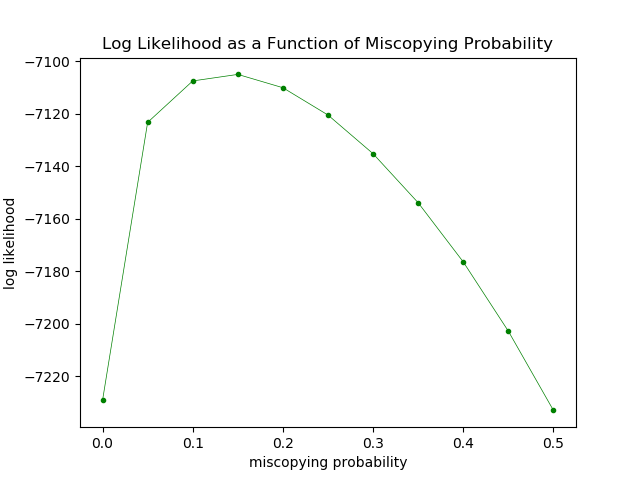
\includegraphics[width=\textwidth]{ceu_gih_5.png}
        \caption{CEU-GIH,$F_{st}=0.031$}
        \label{fig:c}
    \end{subfigure}
    \vfill
    \begin{subfigure}{0.45\textwidth}
        \centering
        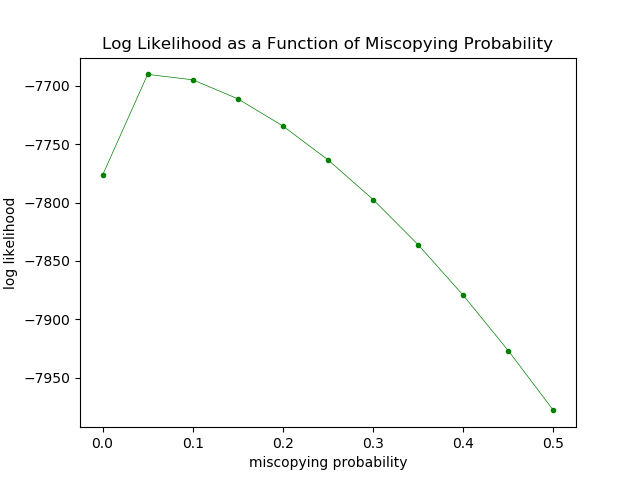
\includegraphics[width=\textwidth]{chd_gih_5.png}
        \caption{CHD-GIH,$F_{st}=0.0768$}
        \label{fig:d}
    \end{subfigure}
    \hspace{1em}
    \begin{subfigure}{0.45\textwidth}
        \centering
        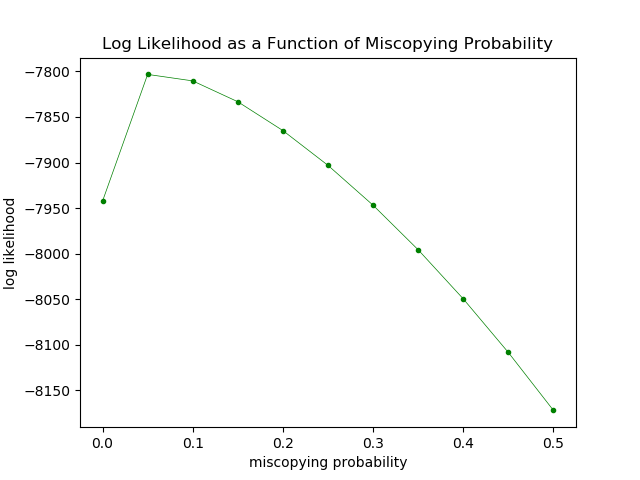
\includegraphics[width=\textwidth]{ceu_chd_5.png}
        \caption{CEU-CHD, $F_{st}=0.1123$}
        \label{fig:d}
    \end{subfigure}
\end{subfigure}
\caption{Hapmix on Admixture between Genetically Similar Ancestral Populations, Log Probability Curve with respect to Miscopying}
\label{fig:logProb}
\end{figure}


Note that the log probability becomes more peaked as $F_{st}$ between the two ancestral populations increases(Fig.\ref{fig:logProb}). With sufficiently large $F_{st}$, the peak is around 0.05, consistent with recommendations stated in \cite{hapmix}.
Several interesting trends can be observed. As expected, the inference accuracy increases as $F_{st}$ between the ancestral population increases. This can also be seen by comparing probability calibration across the four $F_{st}$ being tested here (Fig.\ref{fig:similarPop}). The posterior probability was not well calibrated for the first two paris of ancestral populations, YRI-LWK, CEU-GIH, (see Fig.\ref{fig:YRI-LWK},Fig.\ref{fig:CEU-GIH}) with relatively small $F_{st}$ (0.008, 0.031, respectively). However, the calibration was almost perfect for CHD-GIH and CEU-CHD with $F_{st}$ 0.0768, 0.1123, respectively (see Fig.\ref{fig:CHD-GIH}, \ref{fig:CEU-CHD}). In addition, the inference accuracy for CHD-GIH and CEU-CHD was comparable to that of CEU-YRI, with average hamming distance below 0.05. This seems to suggest that Hapmix should output adequately accurate results when $F_{st} > 0.07$ with reasonably small $T$.
    
     \begin{figure}[H]
     \centering
     \begin{subfigure}[b]{0.45\textwidth}
         \centering
         \includegraphics[width=\textwidth]{YRI-LWK.png}
         \caption{YRI-LWK, $F_{st}=0.008$}
         \label{fig:YRI-LWK}
     \end{subfigure}
     \hfill
     \begin{subfigure}[b]{0.45\textwidth}
         \centering
         \includegraphics[width=\textwidth]{CEU-GIH.png}
         \caption{CEU-GIH, $F_{st}=0.0310$}
         \label{fig:CEU-GIH}
     \end{subfigure}
     \vfill
     \begin{subfigure}[b]{0.45\textwidth}
         \centering
         \includegraphics[width=\textwidth]{CHD-GIH.png}
         \caption{CHD-GIH, $F_{st}=0.0768$}
         \label{fig:CHD-GIH}
     \end{subfigure}
     \hfill
     \begin{subfigure}[b]{0.45\textwidth}
         \centering
         \includegraphics[width=\textwidth]{CEU-CHD.png}
         \caption{CEU-CHD, $F_{st}=0.1123$}
         \label{fig:CEU-CHD}
     \end{subfigure}
        \caption{Posterior Probability Calibration for Hapmix Run under Ancestral Populations with Varying Degree of Divergence}
        \label{fig:similarPop}
\end{figure}
    

It is a bit strange to see that the probability calibration in this setting was much better than that obtained for CEU-YRI admixture. I suspect this to be the result of $\mu$. For CEU-YRI, admixed haplotypes were simulated with $\mu=0.2$, while admixed haplotypes presented in this section were all simulated with $\mu=0.5$. See the next section for a simulation experiment about this.

\subsection{Posterior Probability Calibration Varies with $\mu$}

As noted above, I suspect that the posterior probability is better calibrated when $\mu$ is closer to 0.5. To confirm this, I simulated admixed haplotypes using CEU and YRI as ancestral populations for $\mu=0.05,0.1,0.15,0.2,0.25,0.3,0.4,0.5$ under $T=5,10,20,50$. Results are shown in Fig.\ref{fig:mu}. Indeed the posterior probability appears better calibrated as $\mu$ gets closer to 0.5. 

\begin{figure}[H]
     \centering
     \begin{subfigure}[b]{0.225\textwidth}
         \centering
         \includegraphics[width=\textwidth]{mu1.png}
         \caption{$\mu=0.05$}
         \label{fig:mu=0.05}
     \end{subfigure}1
     \hfill
     \begin{subfigure}[b]{0.225\textwidth}
         \centering
         \includegraphics[width=\textwidth]{mu2.png}
         \caption{$\mu=0.1$}
         \label{fig:mu=0.1}
     \end{subfigure}
     \hfill
     \begin{subfigure}[b]{0.225\textwidth}
         \centering
         \includegraphics[width=\textwidth]{mu3.png}
         \caption{$\mu=0.15$}
         \label{fig:mu3}
     \end{subfigure}
     \hfill
     \begin{subfigure}[b]{0.225\textwidth}
         \centering
         \includegraphics[width=\textwidth]{mu4.png}
         \caption{$\mu=0.2$}
         \label{fig:mu4}
     \end{subfigure}
     \vfill
     \begin{subfigure}[b]{0.225\textwidth}
         \centering
         \includegraphics[width=\textwidth]{mu5.png}
         \caption{$\mu=0.25$}
         \label{fig:mu=0.25}
     \end{subfigure}
     \hfill
     \begin{subfigure}[b]{0.225\textwidth}
         \centering
         \includegraphics[width=\textwidth]{mu6.png}
         \caption{$\mu=0.3$}
         \label{fig:mu=0.3}
     \end{subfigure}
     \hfill
     \begin{subfigure}[b]{0.225\textwidth}
         \centering
         \includegraphics[width=\textwidth]{mu7.png}
         \caption{$\mu=0.4$}
         \label{fig:mu4}
     \end{subfigure}
     \hfill
     \begin{subfigure}[b]{0.225\textwidth}
         \centering
         \includegraphics[width=\textwidth]{mu8.png}
         \caption{$\mu=0.5$}
         \label{fig:mu8}
     \end{subfigure}
        \caption{Posterior Probability Calibration for Hapmix Run under Varying $\mu$}
        \label{fig:mu}
\end{figure}




\subsection{Model Misspecification}
\subsubsection{Effect of Misspecified $\mu$}

Results of running Hapmix with misspecified genome-wide ancestry proportion of CEU $\mu$ is summarized in Table.\ref{tab:misMU} with the bold line indicating results obtained using the true $\mu=0.2$. It can be seen that mis-specified $\mu$ only has minimal, if any, effect on inference accuracy. So Hapmix is very robust with respect to mis-specified $\mu$. One interesting thing to note is that, it appears that the true $\mu=0.2$ doesn't always give the lowest average hamming distance. I believe this is primarily driven by randomness in simulation.

\begin{table}[H]
\begin{center}
\begin{tabular}{ c | c c c c }
\mu & $t=6$ & $t=20$ & $t=50$ & $t=100$ \\
\hline
0.1 & 0.0026 & 0.0072  & 0.0160  & 0.0318 \\
\textbf{0.2} & \textbf{0.003}  & \textbf{0.0073}  & \textbf{0.01555} & \textbf{0.0301}\\
0.3 & 0.003  & 0.0072  & 0.0154  & 0.0290\\
0.4 & 0.003  & 0.0072  & 0.0152  & 0.0281 \\
0.5 & 0.0031 & 0.0072  & 0.0150  & 0.0275\\
0.6 & 0.003  & 0.0071  & 0.0148  & 0.0269
\end{tabular}
\end{center}
\caption{Average Hamming Distance between Inferred and True Local Ancestry for Hapmix with mis-specified $\mu$ under various $T$}
\label{tab:misMU}
\end{table}



\subsubsection{Effect of Misspecified $T$}

To explore the effect of misspeicfied $T$ on the accuracy of inferred local ancestry, I simulated two new sets of 100 admixed haplotypes, one under $T=6,\mu=0.2$, the other under $T=100,\mu=0.2$ again using CEU and YRI as the reference ancestral population. My goal here is to explore how up-biased input $T'$ and down-biased input $T'$ affect inference accuracy respectively.

The 100 admixed haplotypes were used as input to Hapmix with miscopying probability being 0.05. In general, the more the specified $T'$ deviates from the true $T$, the less accurate the inferred local ancestry will be (see Table.\ref{tab:misT} for results obtained when true $T=6,100$, respectively. Bold entries indicate results obtained when $T'=T$). From empirical results I obtained in this set of simulation, Hapmix seems relatively robust when the given $T'$ is within several factors($\sim 5$) of the true $T$. A close look at the posterior probability vs. true ancestry plot (images can be found in the github repo), when true $T$ is small, a large $T'$ introduces many short false positive ancestry switches; when true $T$ is large, a small $T'$ flags many true ancestry switches as false positive. These observations are consistent with the biological meaning of $T$ in the transition model.

\begin{table}[H]
\begin{center}
\begin{tabular}{c | c c c c c c c c c}
true T & $T'=2$ & $T'=6$ & $T'=10$ & $T'=20$ & $T'=30$ & $T'=50$ & $T'=75$ &$T'=100$ & $T'=200$ \\
\hline
$T=6$ & 0.0031 & \textbf{0.0038} & 0.0042 & 0.0046 & 0.0051 & 0.0059& N.A& 0.0081 & 0.0111\\
$T=100$ & 0.0552 & 0.0478 & 0.0416 & 0.0375 & 0.0351 & 0.0321 & 0.0305 & \textbf{0.0296} & N.A
\end{tabular}
\end{center}
\caption{Average Hamming Distance between Inferred and True Local Ancestry for Hapmix with mis-specified $T'$ under true $T=6,100$, sample size=100}
\label{tab:misT}
\end{table}


\subsubsection{Reference Panel Deviates from Real Ancestral Population}

In practice, the ancestral populations might be unknown or extinct, which presents additional challenges to local ancestry inference. I additiaonlly downloaded SNP array data for Luhya in Webuye, Kenya(LWK) and Toscani in Italia (TSI). Admixed individuals were still simulated with CEU and YRI, using the same procedure as described before. To evaluate how Hapmix performs under inaccurate ancestral reference populations, LWK and TSI were used as reference panel to infer local ancestry of CEU-YRI admixed haplotypes. In addition, I also tested Hapmix's performance when one of the two ancestral populations are accurately specified, using CEU-LWK and TSI-YRI as the reference panel. See Table.\ref{tab:misRef} for details.

\begin{table}[H]
\begin{center}
\begin{tabular}{  c| c c c c c c c}
Reference Panel &$T=6$ & $T=20$ & $T=50$ & $T=100$ & \\
\hline
TSI-LWK & 0.0025 & 0.0091 & 0.0200 & 0.0343 & \\
CEU-LWK & 0.0024 & 0.0087 & 0.0190 & 0.0342 & \\
TSI-YRI & 0.0041 & 0.0099 & 0.0189 & 0.0316 & \\
CEU-YRI(baseline)& 0.0027 & 0.0081 & 0.0170 & 0.0300
\end{tabular}
\end{center}
\caption{Average Hamming Distance between Inferred and True Local Ancestry for Hapmix Run under Inaccurately Specified Ancestral Populations}
\label{tab:misRef}
\end{table}

It can be seen that Hapmix performs equally well under this settings compared to the case when accurate ancestral population are specified (row 4). That said, I would expect the accuracy of Hapmix being dependent upon the similarity between the real ancestral population and the mis-specified reference panel. As long as they are reasonably close, Hapmix should be able to produce high-quality local ancestry inference. Indeed, the $F_{st}$ of (TSI, CEU) and (LWK, YRI) are $0.004(0.0001)$, $0.008(0.0001)$, respectively (standard deviation indicated inside parenthesis), based on estimates provided by Hapmap3 \cite{hapmap3}, which indicates that they are more than adequately similar.

It might be interesting to note that, replacing CEU with TSI in the reference panel (row 1 and 2 in Table.\ref{tab:misRef}) only has minimal effect on inference accuracy. This can be explained by the very small $F_{st}$ between CEU and TSI, and, as suggested in \cite{hapmap3} based on their PCA analysis, \say{for many purposes the populations of European ancestry can be grouped together (CEU+TSI)}. 

It is counter-intuitive, however, to note that, replacing LWK with YRI in the inference panel results in lower accuracy when $T=6,20$ (see row 1 and 3 in Table.\ref{tab:misRef}). From $F_{st}$ and PCA analysis, Hapmap3 claims that \say{since the level of admixture in LWK is relatively slight, it may be acceptable to
group LWK with YRI in some analyses} \cite{hapmap3}. It remains unclear to be as of now whether this is due to stochastic effect in simulations or rooted in some deeper factors. 



\section{Discussion}
    This has been a fun project so far, partly because I chose this topic on my own and really thought local ancestry an interesting topic. I originally intended to do something related to coalescent theory (such as ASMC\cite{ASMC}, MSMC\cite{MSMC}, SMC++\cite{SMC++}), yet after reading several papers on this I realized, as Amy has said, they are all too difficult. Luckily, Hapmix turned out just equally interesting.
    
    There are several obvious extensions to Hapmix. It can be made to infer multi-way admixture (as has been done in \cite{1000Genome}), or to allow inference of multiple admixture event between two populations (maybe more suitable for structured coalescent instead). A more ambitious idea is to infer local ancestry in a "unsupervised" fashion, as mentioned by Amy in class. This sounds somewhat reminiscent of STRUCTURE\cite{STRUCTURE} where the $Z$ matrix is used to designate the population origin of each allele copy. The caveat is that STRUCTURE assumes each allele is independent of one another. To model dependence among adjacent SNP sites, the RFMix\cite{RFMix} uses linear-chain conditional random field. In the section titled "Incorporating Information from Admixed Individuals" in RFMix\cite{RFMix} seems to provide some hints for doing so, where they incorporate information from admixed individuals into the reference panel using a EM approach, with initial values provided by the random forest in the first step. In fact, the authors of RFMix explicitly mentioned this in their discussion section. They proposed using ADMIXTURE\cite{ADMIXTURE} to identify admixed individuals having the greatest proportion of each ancestry and use those as the initial proxies for ancestral populations in the EM updates. I wonder how this algorithm would perform if the initial value is randomly assigned. In addition to that, it might also be worth exploring whether a boosting algorithm (instead of a bagging approach, random forest, used in RFMix) would be more suitable during the M step for updating $\theta^A$. 

    
\section{Data and Code Availability}

All code can be found at \url{https://github.com/hyl317/CS4775_FinalProject}. Figures not displayed in this write-up can be found at \url{https://drive.google.com/drive/folders/1oXYQTo68l9PbB_DrnzzZ7Qs5L-OtTcZs?usp=sharing}. They are posterior probability vs. true ancestry plot as in Fig.\ref{fig:posterior}. Those shown in Fig.\ref{fig:posterior} were selected from them as representatives. A brief usage manual can also be found in the README in the github repo. Specification of file format of .snp and .phgeno can be found at \url{https://github.com/williamslab/admix-simu}.

The script insert\_map.pl in the directory ./formatConversion was not written by me. It was downloaded from \url{https://github.com/CNSGenomics/impute-pipe/blob/master/exe/insert-map.pl}. All other scripts were written on my own.

\begin{thebibliography}{9}
\bibitem{hapmix} 
Alkes L. Price et al.
\textit{Sensitive Detection of Chromosomal Segments of Distinct Ancestry in Admixed Populations}. 
Plos Genetics, 2009.
 
\bibitem{Li and Stephen} 
N. Li and M. Stephens. 
\textit{Modeling Linkage Disequilibrium and Identifying Recombination Hotspots Using Single-Nucleotide Polymorphism Data}.
Genetics 165:2213-2233, December 2003.
 
\bibitem{hapmap3} 
The International HapMap 3 Consortium,
\textit{Integrating common and rare genetic variation in diverse human populations}.
Nature, September 2010.


\bibitem{1000Genome}
The 1000 Genomes Project Consortium
\textit{An integrated map of genetic variation from 1,092 human genomes}.
Nature, October 2012.

\bibitem{ASMC}
Pier F. Palamara et al.
\textit{High-throughput inference of pairwise coalescence times identifies signals of selection and enriched disease heritability}.
Nature Genetics, August 2018.

\bibitem{MSMC}
Stephan Schiffels and Richard Durbin. 
\textit{Inferring human population size and separation history from multiple genome sequences}.
Nature Genetics, June 2014.

\bibitem{SMC++}
J. Terhorst et al. 
\textit{Robust and scalable inference of population history from hundreds of unphased whole genomes}
Nature Genetics, February 2017.

\bibitem{STRUCTURE}
Pritchard JK, Stephens M, Donnelly P.
\textit{Inference of population structure using multilocus genotype data}
Genetics. 2000 Jun;155(2):945-59.

\bibitem{RFMix}
Maples, Brian K., et al.
\textit{RFMix: A Discriminative Modeling Approach for Rapid and Robust Local Ancestry Inference}
The American Journal of Human Genetics 93, 278-288, August 8, 2013.

\bibitem{ADMIXTURE}
D.H. Alexander, J. Novembre, and K. Lange.
\textit{Fast model-based estimation of ancestry in unrelated individuals}. 
Genome Research, 19:1655–1664, 2009.

\end{thebibliography}

\end{document}
